\chapter{REVISÃO DE LITERATURA}\label{chap:fundamentacaoTeorica}

Para o presente trabalho, em decorrência dos instrumentos e sensores escolhidos, devemos colher na literatura as equações e formalismos que descrevem o movimento e a orientação dos corpos no espaço, bem como as relações com as forças envolvidas. Além da literatura básica sobre mecânica~\cite{Goldstein1980}, robótica ~\cite{Craig2014} e controle ~\cite{Ogata2010}, os temas são mais bem explorados na literatura sobre controle de aeronaves e mísseis~\cite{Henderson1997}, \cite{Stevens2016}, \cite{Blakelock1991} ou sobre navegação inercial~\cite{Stovall1997}, \cite{Weston2004}, \cite{Wang2021} e~\cite{Haoran2019}.

No particular, empregaremos em grande parte as convenções e equações utilizadas em~\cite{Stevens2016}, que acreditamos dar um tratamento mais direto e acessível a esses temas.

\section{Notação e convenções}

Neste trabalho utilizamos um modelo de mundo tridimensional e mecânica clássica.  Nosso espaço é estruturado por três eixos ortogonais \(x\), \(y\), \(z\) (\(1, 2, 3\)) onde uma posição é dada por um vetor tridimensional. Descreveremos a atitude e o movimento de um corpo rígido sobre a superfície oblata e girante da Terra. Não obstante, serão empregadas aproximações sobre uma pequena área para uma Terra plana, estacionária e constante, que basta\footnotemark{} para os nossos propósitos. Para simbologia, acompanhamos \cite{Stevens2016}:

\begin{align*}
    \mathbf{p}_{A/B} &\equiv
    \text{ vetor posição do ponto A em relação ao ponto B} \\
    \mathbf{v}_{A/i} &\equiv
    \text{ vetor velocidade do ponto \(A\) tomada no sistema \(F_{i}\)} \\
    ^{b}\mathbf{\dot{v}}_{A/i} &\equiv
    \text{ vetor derivada de \(\mathbf{v}_{A/i}\) tomada no sistema \( F_{b}\)} \\
    \mathbf{v}^{c}_{A/i} &\equiv \left( \mathbf{v}_{A/i} \right)^{c} \equiv
    \text{ conjunto dos componentes de \(\mathbf{v}_{A/i}\) expressos no sistema \(c\)} \\
\end{align*}

Componentes de vetores terão índices para indicar o sistema de coordenadas ou serão denotados pelo símbolo de vetor com índices \(x\), \(y\), e \(z\) para indicar as coordenadas, exceto quando indicado pelo símbolo transposto, e todos vetores são do tipo vetor coluna. Acompanhando~\cite{Stevens2016}, por exemplo:
\begin{align*}
    &\mathbf{p}^{b}_{A/B} = \begin{bmatrix}x_{b} \\ y_{b} \\ z_{b}\end{bmatrix}&
    \text{ ou }&
    &\mathbf{v}^{b}_{A/i} = \begin{bmatrix} v_{x} \\ v_{y} \\ v_{z} \end{bmatrix} = \begin{bmatrix} v_{x} & v_{y} & v_{z} \end{bmatrix}^{T}
\end{align*}

\footnotetext{A título de advertência, o assunto não é simples, com diversos formalismos possíveis, um campo fértil para confusão. Por exemplo, a atitude de um corpo pode ser descrita em três dimensões com ângulos de Euler ao menos em doze sequências de rotações anti-horárias distintas, não intercambiáveis, ou ainda pode ser descrita em quatro dimensões com o uso do quaternion, conforme observamos em~\cite{Henderson1997}. Além disso, é importante separar a orientação relativa do nosso espaço tridimensional em abstrato, do eixo de referência em relação ao nosso espaço abstrato, e do sistema móvel que pretendemos descrever em relação ao sistema de referência. No presente trabalho adotaremos um único formalismo que atende aos nossos propósitos limitados, e remetemos o leitor às fontes para aprofundamento do assunto.}

\section{Descrevendo a atitude de um corpo}

Descrevemos a atitude de um robô em ângulos de Euler na sequência \(z\), \(y\), \(x\) (3, 2, 1) que leva de um sistema de referência fixo na Terra até um sistema fixo no corpo do robô. Escolhemos o sistema (\(ned\)) - ``North-East-Down'' (Norte, Leste, Abaixo) com o eixo \(x\) apontando par o Norte, o eixo \(z\) Abaixo, o eixo \(y\) completando o sistema de coordenadas, e o sistema (\(frd\)) - ``Front-Right-Down'' (Avante, Direita, Abaixo), fixo no robô, com eixos, respectivamente, (\(x\),\(y\),\(z\)), sendo o Avante alinhado à \emph{linha de referência longitudinal} do robô, com ``Avante'' e ``Abaixo'' situados no plano de simetria, e o eixo Direito completando o sistema. Adotamos, ainda a convenção de rotações anti-horárias (regra da mão direita).

Desse a modo, a sequência de rotações que leva do sistema de referência \(ned\) para o sistema \(frd\) no corpo é dada por:
\begin{enumerate}
    \item Rotação anti-horária sobre eixo \(z\), ou \(\psi\) positivo (\textit{``compass heading''})
    \item Rotação anti-horária sobre novo eixo \(y'\), ou \(\theta\) positivo (\textit{pitch})
    \item Rotação anti-horária sobre novo eixo \(x''\), ou \(\phi\) positivo (\textit{roll})
\end{enumerate}

Esta sequência de rotações é normalmente denominada \emph{``yaw, pitch, roll''} (guinada, arfada e rolagem), partindo do sistema de referência.

Podemos escrever as matrizes de rotação abreviando co-seno por \(c\) e seno por \(s\). Esta matriz representa uma transformação padrão que será utilizada ao longo do texto, acompanhando~\cite{Stevens2016}:

\begin{align*}
    C_{f\!r\!d\!/\!n\!e\!d} =
    \begin{bmatrix}
        1               &  0            &  0             \\
        0               &  \cos{\phi}   &  \sin{\phi}    \\
        0               & -\sin{\phi}   &  \cos{\phi}
    \end{bmatrix}
    \begin{bmatrix}
        \cos{ \theta}   &  0            & -\sin{\theta} \\
        0               &  1            &  0            \\
        \sin{ \theta}   &  0            &  \cos{\theta}
    \end{bmatrix}
    \begin{bmatrix}
        \cos{\psi}      &  \sin{\psi}   &  0             \\
       -\sin{\psi}      &  \cos{\psi}   &  0             \\
        0               &  0            &  1
    \end{bmatrix}
\end{align*}
\begin{align} \tag{1.3-10}
    C_{f\!r\!d\!/\!n\!e\!d} &=
    \begin{bmatrix}
        c\theta c\psi   & c\theta s\psi & -s\theta    \\
        \left(-c\phi s\psi + s\phi s\theta c\psi \right)
        &  \left( c\phi c\psi + s\phi s\theta s\psi \right)
        &  s\phi c\theta                                 \\
        \left( s\phi s\psi + c\phi s\theta c\psi \right)
        &  \left( -s\phi c\psi + c\phi s\theta s\psi \right)
        & c\phi c\theta
    \end{bmatrix}
\end{align}

O intervalo de validade para o qual os ângulos de rotação são bem definido\footnotemark{} é:
\begin{align*}
    -\pi  < \phi \leq \pi \\
    -\frac{\pi}{2} \leq \theta \leq \frac{\pi}{2} \\
    -\pi < \psi \leq \pi
\end{align*}

\footnotetext{A título de exemplo, ponderamos que caso o ângulo \( \theta \) fosse definido no intervalo de \( \pm 180^{\circ} \) o veículo estaria apontando para o Sul com os ângulos \(\phi\) e \(\psi\) em \( 0^{\circ}\) o que é indesejável pois pode confundir a interpretação.}

\section{Cinemática Rotacional}

Aqui definiremos a derivada de um vetor, mostraremos como ela depende do sistema de referência do observador, e relacionamos as derivadas de um vetor, tomadas em dois sistemas de referência distintos, através do vetor velocidade angular relativa entre esses dois sistemas.

Genericamente a derivada de um vetor é similar à de um escalar~\cite{Stevens2016}:
\begin{equation*}
    \frac{\mathrm{d}}{\mathrm{d}t} \mathbf{p}_{A/B} =  \lim_{\delta t \rightarrow 0 } \begin{bmatrix}
        \displaystyle\frac{\mathbf{p}_{A/B} (t + \delta t) - \mathbf{p}_{A/B} (t) }{\delta t}
    \end{bmatrix}
\end{equation*}

Este novo vetor decorre das mudanças de módulo e orientação de \(\mathbf{p}_{A/B}\). Sendo \(\mathbf{p}\) um vetor livre (por exemplo, a velocidade) sua derivada independe de sua posição, e as mudanças de comprimento e direção decorram do movimento da ponta de \(\mathbf{p}\) em relação à própria cauda. Seja \(\mathbf{p}\) seja um vetor vinculado a algum sistema (por exemplo, o vetor posição) sua derivada naquele sistema é um vetor livre que corresponde à ponta de \(\mathbf{p}\).

\subsection{Velocidade Angular como Vetor}

Um vetor pode apontar em qualquer direção por meio de uma simples rotação ao longo de um eixo apropriado. A fórmula para essa rotação é descrita em~\cite{Goldstein1980}:

\begin{figure}[h]
    \centering
    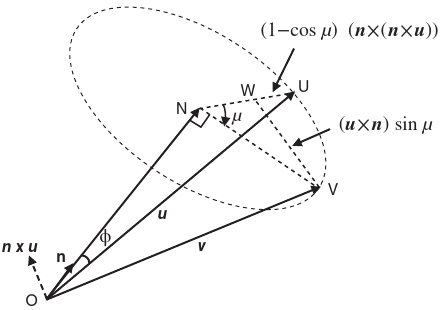
\includegraphics[width=0.5\textwidth, keepaspectratio]{figuras/figure1.2-1.png}\label{fig1.2-1}
    \caption{Rotação de um vetor}\label{fig:rotacao-de-um-vetor}
\end{figure}

Na figura acima, o vetor \(\mathbf{u}\) foi rotacionado para formar o vetor \(\mathbf{v}\) ao definirmos um eixo de rotação ao longo do vetor \(\mathbf{n}\) e realizarmos uma rotação pelo ângulo \(\mu\) ao redor de \(\mathbf{n}\). Estes dois vetores se somam a \(\mathbf{u}\) para obtermos \(\mathbf{v}\), e onde temos que:
    \begin{align*}
     \mathbf{v} &= \mathbf{u} + \left(1 - {\cos{\mu}}\right) \left(\mathbf{n}\!\times\!\left(\mathbf{n}\!\times\!\mathbf{u}\right)\right) - \left(\mathbf{n}\!\times\!\mathbf{u}\right){\sin{\mu}} \tag{1.2-5a}
    \end{align*}
    \begin{align*}
     \mathbf{v} = \left(1 - {\cos{\mu}}\right) \mathbf{n}\!\left(\mathbf{n}\cdot\mathbf{u}\right) + \mathbf{u}{\cos{\mu}} - \left(\mathbf{n}\!\times\!\mathbf{u}\right){\sin{\mu}} \tag{1.2-5b}
    \end{align*}

    As equações acima (1.2-5), às vezes chamadas de \textit{fórmula de rotação}, nos mostram que definindo \(\mathbf{n}\) e \(\mu\) podemos operar sobre \(\mathbf{u}\) com produtos escalares e vetoriais para obter a rotação desejada, independente de sistemas de coordenadas ou magnitude do ângulo.

    Partindo da figura acima, fazemos uma rotação muito pequena \(\delta\mu \ll 1 \text{rad}\), definindo \(\mathbf{v} = \mathbf{u} + \delta \mathbf{u}\), e, aplicando a equação (1.2-5\(a\)) obtemos:
\begin{equation*}
    \delta \mathbf{u} \approx -\!\sin(-\delta\mu)\mathbf{n}\!\times\!\mathbf{u} \approx (\mathbf{n}\!\times\!\mathbf{u})\delta\mu
\end{equation*}

Dividindo por \(\delta t\), no limite onde \(\delta t \rightarrow 0\), definindo \(\mathbf{\omega} \equiv \dot{\mu}\mathbf{n}\), obtemos:

\begin{equation*}
    \dot{\mathbf{u}} = \mathbf{\omega}\!\times\!\mathbf{u}\tag{1.4-1}
\end{equation*}

Esta equação relaciona a velocidade translacional da ponta do vetor \(\mathbf{u}\) ao vetor \(\mathbf{\omega}\). Este vetor \(\mathbf{\omega}\), que denominados \textit{vetor velocidade angular}, constitui-se de um vetor unitário  que define o eixo de rotação, multiplicado pela taxa de rotação. Este é um vetor livre, pode ser trasladado paralelo a si mesmo, e axial, que mudaria de direção caso houvéssemos escolhido uma convenção de sentido horário para a rotação.

Dessa forma podemos associar \(\mathbf{\omega}\) ao sistema de coordenadas fixado no corpo, atribuindo índices que indicam que ele representa a velocidade angular do corpo em relação a outro determinado sistema.

Como vimos, a atitude de um corpo rígido pode ser descrita por uma matriz rotacional variante no tempo, e, pelo teorema de Euler\footnotemark{}, esse o corpo possui um único \emph{eixo instantâneo de rotação} ao qual o vetor velocidade angular é paralelo, e também único.

\footnotetext{\emph{``Euler's Theorem: The general displacement of a rigid body with one point fixed is a rotation about some axis.''} Para uma explicação a respeito, vide~\cite{Goldstein1980}, Capítulo 4.}

\section{Cinemática e Ângulos de Euler}

Um corpo em movimento pode mudar sua atitude, descrita em ângulos de Euler, ao longo do tempo, e neste sentido podemos falar de uma taxa de mudança de cada um desses ângulos de Euler ao longo do tempo. Essas taxas são coisa distintas, é preciso dizer, do vetor velocidade angular do corpo.

Para vincular as taxas de ângulos de Euler, que descrevem a mudança de atitude de um corpo, à sua velocidade angular, procedemos do seguinte modo. Definimos um quadro de referência \(F_{r}\) e um quadro do corpo \(F_{b}\) com vetor velocidade angular relativa \(\omega_{b/r}\) e uma sequencia de ângulos de Euler que define a atitude do corpo, ou seja, a orientação do sistema de coordenadas preso ao corpo em relação ao sistema de referência. Cada taxa de ângulos de Euler informa a direção e magnitude para um determinado vetor velocidade angular sobre um eixo de coordenadas em particular. Esses três vetores somados formam o vetor velocidade angular resultante do veículo cujas taxas de ângulos de Euler estamos tratando. Desse modo podemos encontrar os componentes do vetor velocidade angular resultante \cite{Stevens2016}.

Em outras palavras, movemos sobre a Terra um sistema de coordenada \(frd\) (\emph{``front'', ``right'', ``down''} - frente, direita, abaixo) preso no corpo, com o sistema \(ned\) (\emph{``north'', ``east'', ``down''} - norte, leste abaixo) fixo no quadro de referência, usando uma sequencia ``yaw-pitch-roll'' de ângulos de Euler do sistema \(ned\) para o sistema \(frd\). No caso das equações de Terra plana o sistema \(ned\) é fixado na Terra, e a velocidade angular relativa é aquela do corpo em relação à Terra. Não trataremos aqui do caso mais geral das equações com seis graus de liberdade onde sistema \(ned\) se move sobre a Terra.

As transformações de coordenadas são~\cite{Stevens2016}:

\begin{align*}
    \mathbf{\omega}^{frd}_{b/r} = \begin{bmatrix} \dot\phi \\ 0 \\0 \end{bmatrix}
    + C_{\phi} \begin{pmatrix}
        \begin{bmatrix} 0 \\ \dot\theta \\ 0 \end{bmatrix}
        + C_{\theta}\begin{bmatrix} 0 \\ 0 \\ \dot\psi \end{bmatrix}
    \end{pmatrix}
\end{align*}

\ldots sendo \(C_{\phi}\) e \(C_{\theta}\)  as rotações (anti-horárias) dos planos por cada ângulo de Euler em particular, conforme equação (1.3-10). Multiplicando as matrizes, teremos:

\begin{align} \tag{1.4-3}
    \mathbf{\omega}^{frd}_{b/r} \equiv \begin{bmatrix} P \\ Q \\ R \end{bmatrix}
    = \begin{bmatrix}
        1 & 0 & -\sin{\theta} \\
        0 & \cos{\phi} & \sin{\phi}\cos{\theta} \\
        0 & -\sin{\phi} & \cos{\phi}\cos{\theta}
    \end{bmatrix}
    \begin{bmatrix}
        \dot\phi \\
        \dot\theta \\
        \dot\psi
    \end{bmatrix}
\end{align}

\ldots sendo \(P\), \(Q\), \(R\), os componentes do vetor velocidade angular do corpo expressos no sistema \(frd\), respectivamente, rolagem (\emph{``roll''}), arfada (\emph{``pitch''}) e guinada (\emph{``yaw''}). A transformação inversa é dada por:

\begin{align} \tag{1.4-4}
    \begin{bmatrix}
        \dot\phi \\
        \dot\theta \\
        \dot\psi
    \end{bmatrix}
    =
    \begin{bmatrix}
        1 & \sin{\phi}\tan{\theta} & \cos{\phi}\tan{\theta} \\
        0 & \cos{\phi} & -\sin{\phi} \\
        0 & \frac{\sin{\phi}}{\cos{\theta}} & \frac{\cos{\phi}}{\cos{\theta}}
    \end{bmatrix}
    \begin{bmatrix}
        P \\ Q \\ R
    \end{bmatrix}
\end{align}

Para simplificar, definimos \(\mathbf{\Phi} \equiv \left[\phi \theta \psi \right]^T \) e reescrevemos  (1.4-4) assim:

\begin{equation} \tag{1.4-5}
    \dot{\mathbf{\Phi}} = H \left( \mathbf{\Phi} \right) \mathbf{\omega}^{frd}_{b/r}
\end{equation}

As equações (1.4-3) e (1.4-4) serão referidas como as equações cinemáticas de Euler, como faz~\cite{Stevens2016}. Note que as matrizes de coeficientes \emph{não são} matrizes ortogonais representando rotações ordinárias de coordenadas. Note ainda que as Equações (1.4-4) e (1.4-4) possuem uma singularidade quando  \(\theta = \pm \frac{\pi}{2}\). Ainda, se essas equações forem utilizadas em uma simulação, as taxas de ângulos de Euler podem integrar para ângulos fora do intervalos de ângulos de Euler, e portanto, seria necessário incluir uma lógica para lidar com essa situação no programa simulador. Não obstante, as equações cinemáticas de Euler são bastante empregadas em simulações.

\section{Derivada de um vetor em sistemas móveis}

Nesta seção deveremos obter as equações gerais para o movimento de um corpo no espaço tridimensional. Para generalizar a derivada de um vetor em relação em sistemas móveis obteremos \(^{a}\dot{\mathbf{p}}\) a partir da figura abaixo:
\begin{figure}[H]
    \centering
    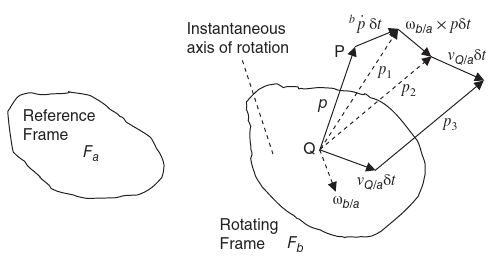
\includegraphics[width=0.5\textwidth, keepaspectratio]{figuras/figure1.4-1.png}\label{fig1.4-1}
    \caption{Derivada de um vetor em sistemas móveis.}
    \fonte{\cite{Stevens2016}}
\end{figure}

Os sistemas \(F_{b}\) e \(F_{a}\) têm velocidade angular relativa \(\mathbf{\omega}_{b/a}\). O ponto \(Q\), fixo em \(F_{b}\), traslada em relação a \(F_{a}\) a uma velocidade \(\mathbf{v}_{Q/a}\). Partindo de  \(Q\) nasce o vetor \(\mathbf{p}\). Observando a partir de \(F_{b}\) estabelecemos \(\mathbf{p}_{1}\) ao acrescentar o efeito \({^b\dot{\mathbf{p}}}\). Olhando a partir de \(F_{a}\) estabelecemos o vetor  \(\mathbf{p}_{2}\) ao somar, ainda, o efeito de \(\mathbf{\omega}_{b/a}\).A partir de \(F_{a}\), estabelecemos \(\mathbf{p}_{3}\) somando o efeito de \(\mathbf{v}_{Q/a}\), que, entretanto, não muda o comprimento ou direção de \(\mathbf{p}_{2}\).Portanto, para obtermos \(^{a}\dot{\mathbf{p}}\) devemos  comparar \(\mathbf{p}_{2}\) a \(\mathbf{p}\) quando \(\delta t \rightarrow 0\). Desse modo, no instante \(\delta t\), \(\mathbf{p}_{2} \!-\! \mathbf{p}\) temos:
\begin{equation*}.
    \mathbf{p}_{2} - \mathbf{p} = {^{b}\dot{\mathbf{p}}} \delta t + \left( \mathbf{\omega}_{b/a} \! \times \!\mathbf{p} \right) \delta t
\end{equation*}

Dividindo por \(\delta t\) no limite em que \(\delta t \rightarrow 0\) resulta na equação\footnotemark{}:
\begin{equation*} \tag{1.4-2}
    {^{a}\dot{\mathbf{p}}} = {^{b}\dot{\mathbf{p}}} + {\mathbf{\omega}_{b/a} \! \times \!\mathbf{p}}
\end{equation*}

\footnotetext{``Equação de Coriolis''~\cite{Stevens2016},~\cite{Blakelock1991}.}

Dentre as propriedades do vetor velocidade angular destacamos\footnotemark{}:
\begin{enumerate}[label=\alph*)]
\item É único e relaciona as derivadas de um vetor tomadas em dois sistemas.
\item Satisfaz a condição de movimento relativo \(\mathbf{\omega}_{b/a} = - \mathbf{\omega}_{a/b}\).
\item É aditivo entre sistemas, ou seja, \(\mathbf{\omega}_{c/a} = \!\mathbf{\omega}_{c/b} + \mathbf{\omega}_{b/a}\) (não vale para aceleração angular).
\item Sua derivada é ambos os sistemas , \({^{a}\dot{\mathbf{\omega}}_{b/a}} = {^{b}\dot{\mathbf{\omega}}_{a/b}} \) .
\end{enumerate}
\footnotetext{Seguindo \cite{Stevens2016}}.

Ainda, derivada de um vetor em um quadro pode ser encontrada a partir das derivadas dos seus componentes expressas em um sistema fixo no mesmo quadro, por exemplo:
\begin{equation*}
    \mathbf{v}^{a\!f} = \begin{bmatrix} v_{x} & v_{y} & v_{z} \end{bmatrix}^{T}
\end{equation*}

\section{Velocidade e Aceleração em quadros móveis}

Encontraremos velocidade e aceleração do ponto \(P\), situado em \(\mathbf{p}\), que se move em relação a \(F_{a}\) e \(F_{b}\), onde fixamos \(O\) and \(Q\), respectivamente, os quais também se movem em relação um ao outro. Na figura abaixo, relacionamos os vetores posição, tomamos suas derivadas no quadro de referência\footnotemark{} \(F_{a}\),  determinando a velocidade. Usando \(\mathbf{v}\) para um vetor velocidade, aplicamos a equação de Coriolis obtendo~\cite{Stevens2016}:
\footnotetext{A escolha do quadro \(F_{a}\) como referência é arbitrária}
\begin{figure}[H]
    \centering
    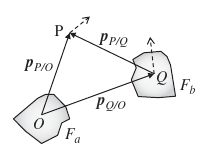
\includegraphics[width=0.25\textwidth, keepaspectratio]{figuras/figure1.5-1.png}
    \label{fig1.5-1}
    \caption{Velocidade e aceleração em quadros móveis}
    \fonte{\cite{Stevens2016}}
\end{figure}
\begin{align}
    \mathbf{p}_{P/O}             &= \mathbf{p}_{Q/O} + \mathbf{p}_{P/Q} \tag{1.5-1} \\
    {^{a}\dot{\mathbf{p}}_{P/O}} &= {^{a}\dot{\mathbf{p}}_{Q/O}} + {^{a}\dot{\mathbf{p}}_{P/Q}} \tag{1.5-2} \\
    \mathbf{v}_{P/a}             &= \mathbf{v}_{Q/a} + \left( \mathbf{v}_{P/b} + \mathbf{\omega}_{b/a}\!\times\!\mathbf{p}_{P/Q} \right) \tag{1.5-3}
\end{align}

Rearranjando para destacar os temos em parênteses\footnotemark{}:
\begin{equation*}
    \mathbf{v}_{P/a} = \mathbf{v}_{P/b} + \left( \mathbf{v}_{Q/a} + \mathbf{\omega}_{b/a}\!\times\!\mathbf{p}_{P/Q} \right),
\end{equation*}
\footnotetext{O termo em parênteses corresponde à chamada \textit{velocidade de transporte de \(P\) no quadro \(F_{a}\)} (a velocidade em \(F_{a}\) de um ponto fixo em \(F_{b}\) coincidente com \(P\)).}

Para a aceleração derivamos (1.5-3) em \(F_{a}\). Velocidades em \(F_{a}\) se tornam acelerações em \(F_{a}\); A velocidade em \(F_{b}\) é derivada pela Equação de Coriolis; A produto vetorial é derivado pela ``regra do produto vetorial''\footnotemark{}; A derivada da velocidade angular é um vetor aceleração angular designado \(\mathbf{\alpha}\). Seja \(\mathbf{a}\) a aceleração translacional em (1.5-3), obtemos:
\begin{equation*}
    \mathbf{a}_{P/a} = \mathbf{a}_{Q/a} + \left(\mathbf{a}_{P/b} + \mathbf{\omega}_{b/a}\!\times\!\mathbf{v}_{P/b}\right) + {{\mathbf{\alpha}_{b/a}}\!\times\!{\mathbf{p}_{P/Q}}} + {\mathbf{\omega}_{b/a}}\!\times\!{\left({\mathbf{v}_{P/b}} + {{\mathbf{\omega}_{b/a}}\!\times\!{\mathbf{p}_{P/Q}}}\right)}
\end{equation*}
\footnotetext{TODO incluir no s anexos a Regra do Produto Vetorial.}

Reorganizando, destacamos aceleração ``\emph{de transporte}'', ``\emph{centrípeta}'' e ``\emph{de Coriolis}'':
\begin{equation*}
    \mathbf{a}_{P/a} = \mathbf{a}_{P/b} + \overbrace{\mathbf{a}_{Q/a} + {{\mathbf{\alpha}_{b/a}}\!\times\!{\mathbf{p}_{P/Q}}} + \underbrace{{{\mathbf{\omega}_{b/a}}\!\times\!{\left({\mathbf{\omega}_{b/a}}\!\times\!{\mathbf{p}_{P/Q}}\right)}}}_{\text{aceleração centrípeta}}}^{\text{aceleração de transporte}} + \underbrace{{2\mathbf{\omega}_{b/a}\!\times\!\mathbf{v}_{P/b}}}_{\text{aceleração de Coriolis}} \tag{1.5-4}
\end{equation*}


Os termos \(\mathbf{a}_{P/a}\) e \(\mathbf{a}_{P/b}\), denominados \emph{aceleração total} e \emph{aceleração relativa}, são expressos nos quadros de referência e secundário, respectivamente. Notamos o surgimento do termo \textit{aceleração de Coriolis}, a ser examinado mais adiante. Se fixamos \(P\) no quadro \(F_{b}\), nos resta apenas \textit{aceleração de  transporte}, definida como a aceleração expressa em \(F_{a}\) de um ponto fixo em \(F_{b}\) instantaneamente coincidente com \(P\). A aceleração de transporte expressa os efeitos do movimento de \(F_{b}\), em termos de aceleração do ponto \(Q\), da velocidade angular e da aceleração angular do quadro~\cite{Stevens2016}.


Por exemplo, um acelerômetro fixo num robô móvel, de corpo rígido, não se move em relação ao quadro do corpo do robô, restando apenas o termo relativos à velocidade e aceleração de transporte nas equações 1.5-3 e 1.5-4, respectivamente. A aceleração para o sensor no ponto \(P\), de posição \(\mathbf{p}_{P/Q}\) em relação a ponto \(Q\) fixo no quadro do robô, denotando \(a\) and \(b\) os quadros de referência e do robô, respectivamente, é dada por \cite{Stevens2016}:
\begin{equation*}
    {\mathbf{a}_{P/a}} = {\mathbf{a}_{Q/a}} + {\mathbf{\alpha}_{b/a}}\!\times\!{\mathbf{p}_{P/Q}} + {\mathbf{\omega}_{b/a}}\!\times\!\left({\mathbf{\omega}_{b/a}}\!\times\!{\mathbf{p}_{P/Q}}\right)
\end{equation*}

Aplicando para um corpo sobre a Terra, sejam \(F_{i}\)  e  \(F_{e}\) quadros de referencia inercial e fixo na Terra, respectivamente, e pontos \(Q\) e \(O\) coincidentes no centro de massa da Terra (sem aceleração translacional), o \(\mathbf{p}_{P/Q}\) é um vetor posição geocêntrico, e \(\mathbf{a}_{Q/a}=0\). Considerando que a Terra gira a uma velocidade angular constante, a derivada de \(\mathbf{\omega}_{b/a}\) também desaparece. Restam a aceleração relativa, a centrípeta e a de Coriolis na equação que relaciona a aceleração verdadeira (inercial) à aceleração relativa, para aplicar as leis de Newton no movimento de um ponto \(P\) sobre a Terra~\cite{Stevens2016}:
\begin{equation*} \tag{1.5-5}
    {\mathbf{a}_{P/i}} = {\mathbf{a}_{P/e}} + {\mathbf{\omega}_{e/i}}\!\times\!\left({\mathbf{\omega}_{e/i}}\!\times\!{\mathbf{p}_{P/O}}\right) + 2\mathbf{\omega}_{e/i}\!\times\!\mathbf{v}_{P/e}
\end{equation*}

Neste sentido, para uma partícula de massa \(m\) situada em \(P\), à aceleração relativa \(\mathbf{a}_{P/e}\) corresponde uma ``força aparente'' sobre a partícula que produz a trajetória vista por um observador estacionário na Terra. À aceleração verdadeira \(\mathbf{a}_{P/i}\) correspondem às `` forças verdadeiras'' (como gravitação e arraste).  Escrevendo (1.5-5) em termos de forças, onde destacamos a \textit{força centrífuga} normal ao vetor velocidade angular, e a \textit{força de Coriolis}\footnotemark{} que fará uma trajetória balística sobre a Terra curvar-se à esquerda ou à direita~\cite{Stevens2016}:
\begin{equation*}
    \text{Força aparente} = \text{força verdadeira} - \underbrace{m \left[{\mathbf{\omega}_{e/i}}\!\times\!\left({\mathbf{\omega}_{e/i}}\!\times\!{\mathbf{p}_{P/O}}\right)\right]}_{\text{força centrífuga}} - \underbrace{m \left( 2{\mathbf{\omega}_{e/i}}\!\times\!{\mathbf{v}_{P/e}}\right)}_{\text{força de Coriolis}}
\end{equation*}

Força verdadeira (\(F\)) é a soma das \textit{forças de contato}. A força do  \textit{campo gravitacional da Terra} corresponde a \(m\mathbf{G}\). O vetor gravidade da Terra (\(g\)) é dado por {\(\mathbf{g}~=~\mathbf{G}~-~\text{aceleração centrípeta}\)}. Desse modo, reescrevendo a equação (1.5-5) para um corpo rígido de massa \(m\), obtemos~\cite{Stevens2016}:
\begin{equation*} \tag{1.5-6}
    \mathbf{a}_{P/e} = \frac{F}{m} + g - {2 \mathbf{\omega}_{e/i}}\!\times\!{\mathbf{v}_{P/e}}
\end{equation*}

\footnotetext{A aceleração de Coriolis será significativa para deslocamento em altas velocidades. Para ilustrar, para que a aceleração de Coriolis tenha a mesma magnitude da aceleração centrípeta, a \(45^{\circ}\) de latitude, um veículo deve deve mover-se a 2365.2 km/h. Nessa velocidade, embora a aceleração de Coriolis ainda seja pequena comparada a \(\mathbf{g}\), causa uma diferença de posição que cresce com o tempo~\cite{Stevens2016}.
\begin{align*}
    &2 \! \begin{vmatrix}{\mathbf{\omega}_{e/i}}\end{vmatrix} \begin{vmatrix}{\mathbf{v}_{cm/e}}\end{vmatrix}\sin\!{\left({45^{\circ}}\right)} = {\begin{vmatrix}{\mathbf{v}_{cm/e}}\end{vmatrix}^{2}} / {r_{E}} \\
    &\begin{vmatrix}{\mathbf{v}_{cm/e}}\end{vmatrix} = {\sqrt{2}}{r_{E}} \begin{vmatrix} {\mathbf{\omega}_{e/i}}\end{vmatrix} \approx 657\text{m/s} \left(2365.2\text{km/h}\right)
\end{align*}
}


\section{Gravitação e acelerômetros}

Um acelerômetro mede, indiretamente\footnotemark{}, a força \(\mathbf{F}\) que equilibra uma \emph{massa de prova} com o encapsulamento. Com o campo gravitacional atuando na massa de prova \(m\), seja \(\mathbf{F}/m\) a força por unidade de massa aplicada à massa de prova, chamada de força específica, \(\mathbf{f}\) determinamos a aceleração \(\mathbf{a}\) da massa de prova~\cite{Stevens2016}:
\begin{equation*}
    \mathbf{a} = \dfrac{\mathbf{F}}{m} + \mathbf{G} \equiv \mathbf{f} + \mathbf{G}.
\end{equation*}
\footnotetext{Para detalhes sobre acelerômetros,~\cite{Weston2004},~\cite{Wang2021} e~\cite{Haoran2019}.}

Com a calibração determinamos o \textit{fator de escala}, entre a quantidade de saída do sinal à força específica\cite{Stevens2016}:
\begin{equation*} \tag{1.6-28}
    \text{Sinal de saída do acelerômetro} = s \mathbf{f} = s \left(\mathbf{a} - \mathbf{G} \right)
\end{equation*}

Quando um acelerômetro, com vetor de posição geocêntrico\footnotemark{} \(\mathbf{p}\), está estacionário em relação à Terra, a leitura de aceleração corresponde a~\cite{Stevens2016}:
\begin{align*}
    \mathbf{a} &= {\mathbf{\omega}_{e/i}}\!\times\!\left({\mathbf{\omega}_{e/i}}\!\times\!{\mathbf{p}}\right) \\
    \mathbf{f} &= \mathbf{a} - \mathbf{G} = -\!{\mathbf{g}} \tag{1.6-29}
\end{align*}
\footnotetext{A navegação inercial exige um modelo para \(\mathbf{G}\) em função da posição. Numa posição diferente, o acelerômetro deve ser corrigido para a gravidade local e pela aceleração centrípeta. Para um acelerômetro fixado em um veículo que se move em relação à Terra, devemos ainda calcular a aceleração de transporte para relacionar a leitura do acelerômetro com a aceleração do veículo~\cite{Stevens2016}.}

Para um acelerômetro com três eixos ortogonais \(x\), \(y\) e \(z\), situado num ponto \({P}\) fixado no quadro \({F}_{frd}\) do corpo de um robô, com vetor de posição geocêntrico \(\mathbf{p}\), designamos \(\mathbf{G}_{p}\) o vetor projeção da força nos elementos sensores, \(\mathbf{g}\) o vetor aceleração da gravidade expresso em múltiplos da \emph{gravidade padrão}, \(\mathbf{a}\) a aceleração do corpo tomada no quadro de referência da Terra, e \({C}_{frd/ned}\) a matriz de rotação do quado \(frd\) em relação ao \(ned\), obtendo a equação:
\begin{equation*}
    {\mathbf{G}}_p = \begin{bmatrix} {G}_{px} \\ {G}_{py} \\ {G}_{pz} \end{bmatrix} = {C}_{frd/ned}\left(\mathbf{g} - {\mathbf{a}}\right)
\end{equation*}

Assumindo que o robô não acelera (\(\mathbf{a}\approxeq0\)) e que na orientação inicial os eixos ``abaixo'' no sistemas \(frd\) e \(ned\) estão alinhados, com o vetor \(\mathbf{g}\) projetando apenas no eixo \(z\) do acelerômetro, então a equação acima se transforma em:
\begin{align*}
    {\mathbf{G}}_p &= \begin{bmatrix}
        c\theta c\psi   & c\theta s\psi & -s\theta    \\
        \left(-c\phi s\psi + s\phi s\theta c\psi \right)
        &  \left( c\phi c\psi + s\phi s\theta s\psi \right)
        &  s\phi c\theta                                 \\
        \left( s\phi s\psi + c\phi s\theta c\psi \right)
        &  \left( -s\phi c\psi + c\phi s\theta s\psi \right)
        & c\phi c\theta
    \end{bmatrix} \begin{bmatrix} 0 \\ 0 \\ 1 \end{bmatrix} = \begin{bmatrix} -\sin{\theta} \\ \cos{\theta}\sin{\phi} \\ \cos{\theta}\cos{\phi} \end{bmatrix}
\end{align*}

A equação acima depende apenas de \(\theta\) e \(\phi\), pois na primeira rotação por \(\psi\) sobre o eixo \emph{abaixo} o vetor \(\mathbf{g}\) permanece alinhado ao eixo \(z\) do sensor. Um acelerômetro, portanto, é insensível a essa rotação por \(\psi\), e não serve para determinar o ângulo de guinada\footnotemark{}. Normalizando as leituras, isolamos \(\theta\) e \(\phi\) por identidades trigonométricas sobre a projeção da gravidade (\(\mathbf{g}\)) nos eixos do sensor~\cite{freescaleAN3461}:
\begin{equation*}
    \frac{{\mathbf{G}}_{p}}{\lVert{{\mathbf{G}}_{p}}\rVert} =
    \frac{1}{\sqrt{{{{G}_{px}}^{2}} + {{{G}_{py}}^{2}} + {{G}_{pz}}^{2}}} \begin{bmatrix} {G}_{px} \\ {G}_{py} \\ {G}_{pz} \end{bmatrix}
    = \begin{bmatrix} -\sin{\theta} \\ \cos{\theta}\sin{\phi} \\ \cos{\theta}\cos{\phi} \end{bmatrix} \\
\end{equation*}
\begin{align*}
    \tan{\phi}_{xyz} &= \frac{G_{py}}{G_{pz}} \\
    \tan{\theta}_{xyz} &= \frac{-G_{px}}{{G_{py}\sin{\phi}}+{{{G}_{pz}}\cos{\phi}}} = \frac{-G_{px}}{\sqrt{{{G_{py}}^{2}}+{{{G}_{pz}}^2}}}
\end{align*}

Empregando funções trigonométricas inversas, obtemos \(\theta\) e \(\phi\):
\begin{align*}
{\phi}_{xyz} &= \tan^{-1}\left(\frac{G_{py}}{G_{pz}}\right) \\
{\theta}_{xyz} &= \tan^{-1}\left(\frac{-G_{px}}{\sqrt{{{G_{py}}^{2}}+{{{G}_{pz}}^2}}}\right) \\
\end{align*}
\footnotetext{Para \(\psi\) poderíamos empregar um magnetômetro~\cite{freescaleAN4248}.}

\ldots e definimos o intervalo de validade\footnotemark{} como fizemos para a matriz rotacional:
\begin{align*}
    -\pi  < \phi \leq \pi \\
    -\frac{\pi}{2} \leq \theta \leq \frac{\pi}{2} \\
\end{align*}
\footnotetext{Nas equações há uma região de instabilidade onde \(\mathbf{G}_{py}\) e \(\mathbf{G}_{pz}\) tendem a zero, quando o eixo \(x\) do acelerômetro encontra-se alinhado verticalmente para cima ou para baixo. Nas proximidades dessa região o cálculo da tangente inversa é dominado pelo ruído do sensor, produzindo uma estimativa de ângulo praticamente aleatória. Fisicamente, quando o eixo \(x\) do acelerômetro está na vertical, o ângulo de rolagem \(\phi\) corresponde a uma rotação sobre o vetor do campo gravitacional, para a qual o acelerômetro é insensível. Algun artifícios podem minimizar a instabilidade~\cite{freescaleAN3461}}

%Ainda sobre o mesmo robô, que não acelera (\(\mathbf{a}\approxeq0\)), mas muda a sua atitude do instante \({t}_{a}\) para \({t}_{b}\), com projeções \(\mathbf{G}_{{p}_{\left[{t}_{a}\right]}\) e \(\mathbf{G}_{{p}_{\left[{t}_{b}\right]}}\), respectivamente, do vetor contante \(\mathbf{g}\) sobre os eixos \(x\), \(y\) e \(z\) do mesmo acelerômetro, estimamos as atitudes \({\Phi}_{\left[{t}_{a}\right]}\) e \({\Phi}_{\left[{t}_{b}\right]}\). Pelo teorema de Euler, aplicamos os produtos escalar e vetorial para estimar o ângulo e o eixo da rotação que leva o vetor \(g\) da projeção \(\mathbf{G}_{{p}_{\left[{t}_{a}\right]}\) à \(\mathbf{G}_{{p}_{\left[{t}_{b}\right]}}\):
%
%\begin{equation*}
%    \mathbf{a} . \mathbf{b} &= \|\mathbf{a}\|\|\mathbf{b}\|\cos{\alpha}\\
%\end{equation*}
%\begin{equation*}
%    \mathbf{a}\times\mathbf{b} &= \|\mathbf{a}\|\|\mathbf{b}\|{\hat{\mathbf{n}}}\sin{\alpha}\\
%\end{equation*}
%
\section{Rigid body dynamics}

In this section we finally put together the ideas and equations fro mthe previous sections to obtain a set of state equations that describe the 6-DoF motion of a rigid aerospace vehicle (defined to be frame \({F}_{b}\)). We shall deal first with the angular motion of the vehicle in response to torques generated by aerodynamic, thrust, or any other forces, whose lines of action do no pass through the vehicle cm. By using the vehicle cm as a reference opint, the rotational dynamics of the aircraft can be separated from the translational dynamics (Wells, 1967): we therefore use a body-fixes corrdinate system, \(bf\), with its origin at the cm to compute moments about the origin. A (nonzero) torque vector produces a rate of change to angular momentum vector, but then, to relate angular momentum to the mass distribution of a specific body, we must use the coordinate system \(bf\) and switch to matrix equations to obtain the components of the angular acceleration vector. Angular acceleration components integrate to angular velocity components, bu then the three degress of freedom in angular displacement are obtained from nonlinear equations such as the Euler equations (1.4-4). For an aircraft, the coordinate system \(bf\) is usually forward-right-down, \(frd\), as described in Section 1.3.
The translational euquations are more straightforward, the acceleration of the vehicle cm is obtained from the vector sum of the various forces, and their lines of action do not have to pass through the cm because th eeffect of any offset is incorporated into the moment equations. The equations are expressed in terms of motion releative to Earth and introduce the usual Coriolis and centripetal terms. Aerodynamic and thrust effects depend on the motion relative to the surrounding atmosphere and so, when the atmosphere is moving relative to Earth, we must introduce an auxiliary equation to compute \emph{relative wind}.

\subsection{Angular Motion}

Here, we develop the equations for the rotational dynamics, which wwill be the same for both the falt-Earth and oblate-rotating-Earth equations of motion. The following definitions will be needed:

\begin{align*}
    {F}_{i} &= \text{ an intertial reference frame} \\
    {F}_{b} &= \text{ the body of the rigid vehicle} \\
    \mathbf{v}_{cm/i} &= \text{ velocity of vehicle cm in }{F}_{i} \\
    \mathbf{\omega}_{b/i} &= \text{ angular velocity of }{F}_{b}\text{ with respect to }{F}_{i} \\
    \mathbf{M} &= \text{ vector sum of all moments about the cm}
\end{align*}

The moment, \(\mathbf{M}\), may be generated by aerodynamic effects, any propulsion-force components not acting through the cm, and attitude control devices.

Let the angular momentum vector of a rigid body in the inertial frame and taken about the cm be denoted by \(\mathbf{h}\). It is shown in thextbooks on classical mechanics (Goldstein, 1980), that the derivative of \(\mathbf{h}\) taken in the inertial frame is equal to the vector moment \(\mathbf{M}\) applied about the cm. Therefore, analogously to Newton's law for translational momentum, we write

\begin{equation}
    \mathbf{M}={^{i}\dot{\mathbf{h}}_{cm/i} \tag{1.7-1}}
\end{equation}

The angular momentum vector can be found by considering an element of mass \(\delta m\) with position vector \(\mathbf{r}\) relative to the cm. Its translational momentum is given by

\begin{equation*}
    \left( \mathbf{v}_{cm/i} + \mathbf{\omega}_{b/i} \times \mathbf{r} \right) \delta m
\end{equation*}

The angular momentum of this particle about the cm is the moment of the translational momentum about the cm, or

\begin{equation*}
    \mathbf{\delta h} = \mathbf{r} \times \left( \mathbf{v}_{cm/i} + \mathbf{\omega}_{b/i} \times \mathbf{r} \right) \delta m
\end{equation*}

And for the whole body

\begin{equation*}
    \mathbf{h}_{cm/i} = \iiint \mathbf{r} \times \left( \mathbf{v}_{cn/i} + \mathbf{\omega}_{b/i} \times \mathbf{r} \right) dm
    \end{equation*}

    In order to integrate this equation over the whole body, we mus choose a coordinate system and, to avoid a time=varying integrand, the coordinate system msut be fixed in the body. Let the position coordinates in body-fixed axes, \(bf\), be

    \begin{equation*}
        \mathbf{r}^{bf} = {\begin{bmatrix} x & y &z \end{bmatrix}}^{T}
    \end{equation*}

    The corresopnding matrix equation for \(\mathbf{h}\) is obtained by replacing the cross-products by \(\mathbf{\tilde{r}}\) and noting that \(\mathbf{v}\) and \(\mathbf{\omega}\) are constants fot the purposes of integration. The first term contains only integrals whose integrands have a position coordinate integrated \(dm\) and, by definition of the dm, they all integrate to zero. The second term is:
    \begin{equation*}
        \mathbf{h}^{bf}_{cm/i} = - \iiint \mathbf{\tilde{r}} \left( \mathbf{\tilde{r}} \mathbf{\omega}^{bf}_{b/i} \right) dm = - \iiint \mathbf{\tilde{r}}^{2} dm \mathbf{\omega}^{bf}_{b/i}
    \end{equation*}

    giving

    \begin{equation*}\tag{1.7-2}
        \mathbf{h}^{bf}_{cm/i} = \iiint \begin{bmatrix}
            \left(y^{2} + z^{2}\right)  & -xy                           & -xz \\
            -xy                         &   \left(x^{2} + z^{2}\right)  & -yz \\
            -xz                         &   -yz                         & \left(x^{2} + y^{2}\right) \\
        \end{bmatrix} dm \mathbf{\omega}^{bf}_{b/i}
    \end{equation*}

    The result of this integration is a \(3 \times 3\) constant matrix that is defined to be the \emph{inertia matrix} \(\mathbf{J}^{bf}\) fot he rigid body; it contains scalar \emph{moments} and \emph{cross-products of inertia}, for example:

    \begin{equation*}
        \text{Moment of Inertia about x-axis} = \mathbf{J}_{xx} = \int{ \left( x^{2} + z^{2} \right)} dm
    \end{equation*}
    \begin{equation*}
        \text{Cross-Product of Inertia } \mathbf{J}_{xy} \equiv \mathbf{J}_{yx} = \int{xy}dm
    \end{equation*}

    and so,

    \begin{equation*}\tag{1.7-3}
        \mathbf{h}^{bf}_{cm/i} = \begin{bmatrix}
             \mathbf{J}_{xx} & -\mathbf{J}_{xy} & -\mathbf{J}_{xz} \\
            -\mathbf{J}_{xy} &  \mathbf{J}_{yy} & -\mathbf{J}_{yz} \\
            -\mathbf{J}_{xz} & -\mathbf{J}_{yz} &  \mathbf{J}_{zz} \\
        \end{bmatrix}
        \mathbf{\omega}^{bf}_{b/i} \equiv \mathbf{J}^{bf} \mathbf{\omega}^{bf}_{b/i}
    \end{equation*}

    It was necessary to choose a coordinate system to obtain this matrix and, consequently, it is not possible to obtain a vector equation of motion that is completely coordinate free. In more advanced treatment, this paradox is avoided by the use of tensors. Note also that \(\mathbf{J}\) is a real symmetric matrix and therefore has special properties that are discussed below. Various formulae and theorems are available for calculating \(\mathbf{J}^{bf}\) for a composite body like an aircraft, and it can be estimated experimentally with the aircraft mounted on a turntable.

    With the angular momentum expressed in terms of the inertia matrix and angular velocity vector of the complete rigid body, Equation (1.7-1) can be evaluated. Since the inertia matrix is knwown, and constant in the body-fram, it will be convenient to replace the derivative in (1.7-1) by a derivative taken in the body frame:

    \begin{equation*}\tag{1.7-4}
        \mathbf{M} = {^{i}{\dot{\mathbf{h}}_{cm/i}}} = {^{b}{\dot{\mathbf{h}}_{cm/i}}} + \mathbf{\omega}_{b/i} \times \mathbf{h}_{cm/i}
    \end{equation*}

    Now, differentiating (1.7-3) in \({F}_{b}\), with \(J\) constant, and taking body-fixed components, we obtain

    \begin{equation*}
        \mathbf{M}^{bf} = \mathbf{J}^{bf} {\dot{\mathbf{\omega}}^{bf}_{b/i}} + {\tilde{\mathbf{\omega}}}^{bf}_{b/i} \mathbf{J}^{bf} \mathbf{\omega}^{bf}_{b/i}
    \end{equation*}

    A rearrangement of this equation gives the \emph{state equation for angular velocity}:

    \begin{equation}\tag{1.7-5}
    {^{b}{\dot{\mathbf{\omega}}^{bf}_{b/i}}} = {\left(\mathbf{J}^{bf}\right)}^{-1}
             \begin{bmatrix} \mathbf{M}^{bf} & - \tilde{\mathbf{\omega}}^{bf}_{b/i} \mathbf{J}^{bf} & \mathbf{\omega}^{bf}_{b/i} \end{bmatrix}
    \end{equation}

    This state equation is widely used in simulation and analysis of rigid-body motion from stellites to ships. It can be solved numerically for the angular velocity given the inertia matrix and the torque vector, and its features will now be described.

    The assumption that the inertia matrix is constant is not always completely true. For example, with aircraft the inertias will change slowly as fuel is transferred and burned. Also, the inertias will change abruptly if an aircraft is engaged in dropping stores. These effects can usually be adequately accounted for in a simulation by simply changing the inertias in (1.7-5) without accounting for their rates of change. As far as aircraft control system design is concerned, point designs are done for particular flight conditions, and interpolation between point designs can be used when the aircraft mass properties change. This is more likely to be done to deal with movement of the vehicle cm and the resultant effect on stability (Chapter 2).
    The inverse of the inertia matrix occurs in (1.7-5), and because of symmetry this has a relatively simple form:
    \begin{equation}\tag{1.7-6}
        \mathbf{J}^{-1} = \frac{1}{\Delta}
        \begin{bmatrix}
            k_{1} & k_{2} & k_{3} \\
            k_{2} & k_{4} & k_{5} \\
            k_{3} & k_{5} & k_{6} \\
        \end{bmatrix}
    \end{equation}

    where

    \begin{align*}
        &k_{1} = \left(\mathbf{J}_{yy} \mathbf{J}_{zz} - \mathbf{J}_{yz}^{2} \right) / \Delta, \\
        &k_{2} = \left(\mathbf{J}_{yz} \mathbf{J}_{zx} + \mathbf{J}_{xy} \mathbf{J}_{zz} \right) / \Delta, \\
        &k_{3} = \left(\mathbf{J}_{xy} \mathbf{J}_{yz} + \mathbf{J}_{zx} \mathbf{J}_{yy} \right) / \Delta, \\
        &k_{4} = \left(\mathbf{J}_{zz} \mathbf{J}_{xx} - \mathbf{J}_{zx}^{2} \right) / \Delta, \\
        &k_{5} = \left(\mathbf{J}_{xy} \mathbf{J}_{zx} + \mathbf{J}_{yz} \mathbf{J}_{xx} \right) / \Delta, \\
        &k_{6} = \left(\mathbf{J}_{xx} \mathbf{J}_{yy} - \mathbf{J}_{xy}^{2} \right) / \Delta, \\
        &\Delta = \mathbf{J}_{xx} \mathbf{J}_{yy} \mathbf{J}_{zz} - 2 \mathbf{J}_{xy} \mathbf{J}_{yz} \mathbf{J}_{zx} - \mathbf{J}_{xx}\mathbf{J}_{yz}^{2} - \mathbf{J}_{yy}\mathbf{J}_{zx}^{2} - \mathbf{J}_{zz}\mathbf{J}_{xy}^{2}
    \end{align*}

    A real symmetric matrix has real eigenvalues and, furthermore, a repeated eigenvalue of order \(p\) still has associated with it \(p\) linearly independent eigenvectors. Therefor, a similarity transformation can be found that reduces the matrix to a real diagonal form. In the case of the inertia matrix this means that we can find a set of coordinate eaxes in which the inertia matrix is diagonal. These axes are called the \emph{principal axes}. The inverse of a diagonal matrix is also diagonal and the angular velocity state equation takes its simples form, knwown as \emph{Euler's equations of motion}.
    At this point it is convenient to be more specific and choose the body-fixed axes to be \(frd\), so thtat we can use the standard aircraft yaw, pitch, and roll symbols:
    \begin{equation}\tag{1.7-7}
        \mathbf{M}^{frd} = {\begin{bmatrix} \ell & m & n \end{bmatrix}}^{T}, \quad
        \mathbf{\omega}^{frd}_{b/i}= {\begin{bmatrix} P & Q & R \end{bmatrix}}^{T}
    \end{equation}

    Then Euler's equations of motion are
    \begin{align*}
        \dot{P} &= \frac{\left( J_{y} - J_{z} \right)}{ Q R}{ J_{x} } + \frac{ \ell }{ J_x } \\
        \dot{Q} &= \frac{\left( J_{z} - J_{x} \right)}{ Q R}{ J_{y} } + \frac{ m    }{ J_y } \\
        \dot{R} &= \frac{\left( J_{x} - J_{y} \right)}{ Q R}{ J_{z} } + \frac{ n    }{ J_z }\tag{1.7-8}
    \end{align*}

    and the double subscript notation on the moments of inertia has been dropped. The equations involve cyclic permutation of the rate and inertia components; they are inherently coupled because angular rates about any two axes produce an angular acceleration about the third. This \emph{inertia coupling} has important consequences for aircraft manueuvering rapidly at high angles of attack; we examine its effects in Chapter 3. The stability properties of the Euler equations are interesting and will be studied in Problem 1.7-3.

    The angular velocity satte equation is again simplified when applied to aircraft since for most aircraft the \(frd\) \(x-z\) plane is a plane of symmetry. Under this condition, for every product \(y_{i} z_{j}\) or \(y_{i} x_{j}\) in an inertia computation there is a product that is identical in magnitude but opposite in sign. Therefore, only the \(J_{xz}\) cross-product of inertia is nonzero. A notable exception is an oblique-wing aircraft (Trvassos et al., 1980), which does not have a plane of symmetry. Under the plane-of-symmetry assumption the inertia matrix and its inverse reduce to

    \begin{align*}\tag{1.7-8}
    J^{frd} &=
    \begin{bmatrix}
         J_{x}   & 0         & -J_{xz}    \\
         0       & J_{y}     &  0         \\
        -J_{xz}  & 0         &  J_{z}     \\
    \end{bmatrix}
    ,\quad
    {\left(J^{frd}\right)}^{-1} = \frac{1}{\Gamma}
    \begin{bmatrix}
         J_{x}   & 0         &  J_{xz}    \\
         0       &\left(\frac{\Gamma}{J_{y}}\right)     &  0         \\
         J_{xz}  & 0         &  J_{z}     \\
    \end{bmatrix} \\
    \Gamma &= J_{x} J_{z} - J^{2}_{xz}
\end{align*}

If the angular velocity state equation (1.7-5) is expanded using yhe torque vector in (1.7-7) and the simple inertia matrix given by (1.7-9), the coupled, nonlinear angular acceleration equations are

\begin{align*}\tag{1.7-10}
    \Gamma \dot{P} &=  J_{xz} \left( J_{x} - J_{y} + J_{z} \right) P Q - \left[ J_{z} \left( J_{z} - J_{y} \right) + J^{2}_{xz} \right] Q R + J_{z} \ell + J_{xz}n \\
J_{y} \dot{Q} &= \left( J_{z} - J_{x} \right) R P - J_{xz} \left( P^{2} - R^{2} \right) + m \\
    \Gamma \dot{R} &= -J_{xz} \left( J_{x} - J_{y} + J_{z} \right) Q R + \left[ J_{x} \left( J_{x} - J_{y} \right) + J^{2}_{xz} \right] P Q + J_{xz} \ell + J_{x}n \\
\end{align*}

In the analysis of angular motion we have so far neglected the angular momentum of any spinning rotors. Technically this violates the rigid-body assumption, but the resulting equations are valid. Note that, strictly, we require axial symmetry of the spinning rotors; otherwise the position of the vehicle cm will vary. This is not a restrictive requirement because it is also a requirement for dynamically balancing the rotors. The effects of the additional angular momentum may be quite significant. For example, a number of World Wai I aircragt had a single ``rotary'' engine that had a fixed crankshaft and rotating cylinders. The gryroscopic effect caused by the large angular momentum of the engine gave these aircraft tricky handling characteristics. In the case of a small jet with a single turbofan engine on the longitudinal axis, the effects are smaller. To represent the effect, a constant vector can be added to the angular momentum vector in (1.7-3); therefore, let

\begin{equation*}\tag{1.7-11a}
    \mathbf{h}^{bf}_{cm/i} = J^{bf} \mathbf{\omega}^{bf}_{b/i} + {{\begin{bmatrix} h_{x} \\ h_{y} \\ h_{z}\end{bmatrix}}_{\text{engines}}}
\end{equation*}

To complete the set of equations for angular motion, anttitude state equation is required. Here, with the flat-Earth equations in mind, we will assume that this will be the Euler kinematical equations (1.4-4). A direction cosine matrix can be computed from the Euler angles and will be needed in the translational equations. Thus, the translational equations will be coupled to the rotational equations. We now have all of the state equations for the angular motion dunamics, and we will turn our attention to the translational motion of the cm.

\subsection{Translational motion of the Center of Mass}

\paragraph{Vector State Equations}
We begin by applying Newton's second lat to the motion of a constant-mass rigid body near the surface of Earth to find the inertial derivative of velocity under the influence of aerodynamic, propulsion, and mass attraction forces. We shall find state equations, in vector form at first, for position and velocity.

Some considerations for the choice of state variables are that the velocity vector can be chosen for convenience in either navigation over Earth or aerodynamic force and moment calculations on the body. The position vector can be taken from an arbitrary fixed point in the rigid-Earth frame, \(F_{e}\). If the variation in gravity is significant over the trajectory, then the position vector should be taken from Earth's cm but will be over six million meters long. For short-range navigation it can more conveniently be taken from an initial point on the surface of Earth, bu then latitude and longitude cannot be easily calculated. We will first derive equations for convenience in navigation using velocity of the vehicle cm in \(F_{e}\) and taking the position vector from Earth's cm.

Earth's cm is a fixed point common to both the inertial frame, \(F_{i}\), and the Earth frame, \(F_{e}\), so the derivative of a position vector from the cm will five either the inertial velocity or Earth velocity, according to the frame in which the derivative is taken. Derivatives in \(F_{i}\) and \(F_{e}\) are related through Earth's angular velocity vector, \(\mathbf{\omega}_{e/i}\), according to the Coriolis equation. In addition to the above frames, the rigid-body frame \(F_{b}\) will be required. We also define the following scalars and vectors:

\begin{align*}
    m &\equiv \text{ Vehicle (constant) mass} \\
    O &\equiv \text{ Earth cm} \\
    \mathbf{p}_{cm/O} &\equiv \text{ Vehicle position relative to }O \\
    \mathbf{v}_{cm/i} &\equiv {^{i}\dot{\mathbf{p}}_{cm/O}} = \text{ Velocity of the cm in }F_{i} \\
    \mathbf{v}_{cm/e} &\equiv {^{i}\dot{\mathbf{p}}_{cm/O}} = \text{ Velocity of the cm in }F_{e}  \\
    \mathbf{\omega}_{x/y} &\equiv \text{ Angular velocity of frame \(x\) with respect to frame \(y\)} \\
    \mathbf{F} &\equiv \text{ Vector sum of forces at cm} \\
    m &\equiv \text{ Earth's gravitation vector} \\
    \mathbf{g} &\equiv \text{ Earth's gravity vector, }\mathbf{g} = \mathbf{G} = \mathbf{omega}_{e/i} \times \left( \mathbf{\omega}_{e/i} \times  \mathbf{p}_{cm/O} \right) \\
\end{align*}

From the above explanation and definition, the position and velocity state equations, in vector form, are

\begin{align*}\tag{1.7-12}
    {^{e}{\dot{\mathbf{p}}}_{cm/O}} = \mathbf{v}_{cm/e} \\
    {^{e}{\dot{\mathbf{v}}}_{cm/e}} = \mathbf{a}_{cm/e} \\
\end{align*}

To apply Newton\'s laws we use Equation (1.5-5), substitute \(\left( \textstyle{\frac{1}{m}}\mathbf{F} + \mathbf{G}\right)\) for the inertial acceleration, and solve for the relative acceleration (i.e., the derivative of the velocity state in \(F_{e}\)):

\begin{equation*}\tag{1.7-13}
    {^{e}{\dot{\mathbf{v}}_{cm/e}}} = \textstyle{\frac{1}{m}} \mathbf{F} + \mathbf{G} - \mathbf{\omega}_{e/i} \times \left( \mathbf{\omega}_{e/i} \times \mathbf{p}_{cm/O} \right) - 2 \mathbf{\omega}_{e/i} \times \mathbf{v}_{cm/e}
\end{equation*}

This velocity state equation together with the position state equation is suitable for accurate simulation of flight around the oblate, rotating Earth. Latitude and longitude and \(\mathbf{G}\) can be calculated from the geocentric position vector. The Coriolis term was examined in Section 1.5; a rule of thumb is to consider the Coriolis effect significant for speeds over about 2000ft/s.

Finally, true airspeed is needed for calculating aerodynamic effects and propulsion system performance; therefor we define a relative velocity vector, \(mathbf{v}_{rel}\), by

\begin{equation*}\tag{1.7-14}
    \mathbf{v}_{rel} = \mathbf{v}_{cm/e} - \mathbf{v}_{W/e} \text{,}
\end{equation*}

where \(\mathbf{v}_{w/e}\) is the wind velocity taken in \(F_{e}\). This is an auxiliary equation that will be needed with the state equations.

The full set of 6-DoF oblate, rotating-Earth matrix equations will be illustrated in Section 1.8 and we will now simplify the vector equations (1.7-12) and (1.7-13) to obtain the much more commonly used \emph{flat-Earth equations}. If the \(\mathbf{g}\) vector can be considered to be independent of latitude and taken to be approximately constant or dependent only on height above Earth's surface, the position vector can be taken from a point of interest, \(Q\), on Earth's surface. The position vector then need no longer be six million meters long, but latitude and longitude cannot be calculated from it, and it will give only approximate distances over Earth's surface. If \(Q\) is the fied point on Earth's surface, then the position state equation is

\begin{equation*}\tag{1.7-15}
    {^{e}{\dot{\mathbf{p}}_{cm/Q}}} = \mathbf{v}_{cm/e}
\end{equation*}

    As noted at the beginning of this section, the velocity state equation can alternatively be expressed in terms of a vector derivative taken in the vehicle body frame, and then when components are taken in a body-fixed coordinate system, we have a set of component derivatives that can be integrated to provide velocity components that determine aerodynamic effects. Changing derivatives in Equation (1.7-13) and substituting for \(\mathbf{g}\), we have

\begin{align*}\tag{1.7-16a}
    {^{b}{\dot{\mathbf{v}}}_{cm/e}} + \mathbf{\omega}_{b/e} \times \mathbf{v}_{cm/e} &= {^{e}{\dot{\mathbf{v}}_{cm/e}}} = \textstyle{\frac{1}{m}}\mathbf{F} + \mathbf{g} - 2 \mathbf{\omega}_{e/i} \times \mathbf{v}_{cm/e} \\
{^{b}{\dot{\mathbf{v}}_cm/e}} &= \textstyle{\frac{1}{m}} \mathbf{F} + \mathbf{g} - \left( \mathbf{\omega}_{b/e} + 2 {\mathbf{\omega}_{e/i}}\right) \times \mathbf{v}_{cm/e}
\end{align*}

Alternatively, using the additive property of angular velocity vectors,

\begin{align*}\tag{1.7-16b}
    {^{b}{\dot{\mathbf{v}}_{cm/e}}} &= \textstyle{\frac{1}{m}} \mathbf{F} + \mathbf{g} - \left( \mathbf{\omega}_{b/i} + \mathbf{\omega}_{e/i} \right) \times \mathbf{v}_{cm/e}
\end{align*}

A further assumption is that Earth is an inertial reference frame; Earth's angular velocity can then be neglected, and \(\mathbf{\omega}_{b/i} \equiv \mathbf{\omega}_{b/e}\), and Equations (1.7-16a) and (1.7-16b) both reduce to

\begin{align*}\tag{1.7-16c}
    {^{b}{\dot{\mathbf{v}}_{cm/e}}} &= \textstyle{\frac{1}{m}} \mathbf{F} + \mathbf{g} - \mathbf{\omega}_{b/e} \times \mathbf{v}_{cm/e}
\end{align*}

These approximations are the basis o the flat-Earth equations of motion, described in the next section.

\subsection{The Flat-Earth Equations, Matrix Form}

As explained above, the flat-Eearth equations are not suitable for precise determination of position over Earth, but they are widely used in simulations to study aircraft performance and dynamic behavior and are used to derive linear state-space models for analytical studies and flight control system design. The assumptions fot the flat-Earth equations will now be formally listed:

\begin{enumerate}
    \item The Earth frame is an inertial reference frame.
    \item Position is measured in a tangent-plane coordinate system, \(tp\).
    \item The gravity vector is normal to the tangent plane and constant in magnitude.
\end{enumerate}

Some consequent assumptions are:

\begin{enumerate}
    \item Height above the tangent plane is a good approximation to true height above Earth's surface, and the horizontal projection of the position vector gives a good approximation to distance traveled over Earth's surface (this will be reasonable up to a few hundred miles from the tangent plane origin).
    \item The attitude of the vehicle in the tangent plane coordinate system is a good approximation to true geographic attitude at the position of the vehicle
\end{enumerate}

Equation (1.7-16) already imposes the first flat-Earth assumption, and the position state variable is already referred to the tangent-plane origin; we must now make choices of coordinate systems for the variables in the state equations and make provisions to calculate a rotation matrix to convert from one system to another where necessary.

A \(frd\) coordinate system fixed in  \(F_{b}\) is very convenient for the velocity vector derivative in \(F_{b}\), for the aerodynamic and propulsion forces, and for the vehicle angular velocity vector (which uses body-axes components in the angular motion equations). This choice is less convenient for the \(\mathbf{g}\) vector and Earth angular velocity vector; these are known in Earth-fixed coordinate systems and must be rotated into the body axes using a vehicle-attitude DCM obtained from the attitude state equations. In the flat-Earth equations, the changing attitude of the vehicle is almost invariably adequately modeled with the simple Euler kinematical equations, (1.4-4). These realte a \(frd\) body-fixed system to a \(ned\) system, here the \(ned\) system is the \emph{tangent plane system}, \(tp\), fixed in the Earth. The Euler angles can then be used to construct the \(C_{frd/tp}\) DCM, which must be done before the position and velocity equations can be evaluated.

The set of 6-DoF state equations will be completed by the addition of the angular velocity state equation (1.7-5), with \(\mathbf{\omega}_{b/i} \equiv \mathbf{\omega}_{b/e}\) as the state variable. The state vector is now

\begin{align*}\tag{1.7-17}
    X^{T} =
    \begin{bmatrix}
    \left( \mathbf{p}^{tp}_{cm/O} \right) &
    \mathbf{\Phi}^{T} {\left(\mathbf{v}^{frd}_{cm/e}\right)}^{T} &
    {\left(\mathbf{\omega}^{frd}_{b/e} \right)}^{T}
    \end{bmatrix}
\end{align*}

Using the values of the state variables we evaluate the state derivatives as follows. The rotation matrix is calculated before the position and velocity state equations as noted above. Aerodynamic angle derivatives can be calculated form the translational velocity derivatives, and therefore the translational velocity state equation is placed ahead of the angular velocity state equations, where those derivatives are more significant (this is explained in detail in Chapter 3) and we have the following set of equations:

\begin{align*}\tag{1.7-18}
    C^{frd/tp} &= fn \left( \Phi \right) \\
    \dot{\Phi} &=  H \left( \Phi \right) {\mathbf{\omega}^{frd}_{b/e}} \\
    {^{e}{\dot{\mathbf{p}}^{tp}_{cm/Q}}} &= {C_{tp/frd}}{\mathbf{v}^{frd}_{cm/e}} \\
    {^{b}{\dot{\mathbf{v}}^{frd}_{cm/e}}} &= \textstyle{\frac{1}{m}} {\mathbf{F}^{frd}} + {C_{frd/tp}}{\mathbf{g}^{tp}} - {\tilde{\mathbf{\omega}}^{frd}_{b/e}} {\mathbf{v}^{frd}_{cm/e}} \\
    { ^{b}{\dot{\mathbf{\omega}}^{frd}_{b/e}}} &= {\left( J^{frd} \right)}^{-1}
    \begin{bmatrix}
        \mathbf{M}^{frd} & -{\tilde{\mathbf{\omega}}^{frd}_{b/e}} {J^{frd}} & {\mathbf{\omega}^{frd}_{b/e}}
    \end{bmatrix}
\end{align*}

The 6-DoF flat-Earth equations contained in (1.7-8) are twelve (scalar) coupled, nonlinear, first-order differential equations and an auxiliary equation. Coupling exists because angular acceleration integrates to angular velocity, which determines the Euler angle rates, which in turn determine the direction cosine matrix. The direction cosine matrix is involved in the state equations for position and velocity; position (the altitude component) and velocity determine aerodynamic effects which determine angular acceleration. Coupling is also present through the translational velocity. These interrelationships will become more apparent in Chapter 2.

To complete the flat-Earth assumptions, \(\amthbf{g}\) in tangent-plane coordinates will be

\begin{equation*}
\mathbf{g}^{tp} = {\begin{bmatrix} 0 & 0& g_{D} \end{bmatrix}}^{T}
\end{equation*}

with the down component, \(\mathbf{g}_{D}\), equal to the standard gravity (\(9.80665 \textrm{m/s}^{2}\)), or the local value. Aerodynamic calculations will require the equation for the velocity vector relative to the surrounding air [from Equation (1.7-14)]:

\begin{equation*}\tag{1.7-19}
    \mathbf{v}^{frd}_{rel} =  \mathbf{v}^{frd}_{cm/e} - \mathbf{C}_{frd/tp} \mathbf{v}^{tp}_{W/e}
\end{equation*}

Some additional auxiliary equations will be needed to compute all of the aerodynamic effect, but these will be introduced in Chapter 2.

An interesting alternative to the translational velocity state equation in (1.7-18) can be derived by using relative velocity as the state variable. The vector form of the relative velocity equation is (1.7-14). If this equation is differentiated in the body-fixed frame and used to eliminate \(\mathbf{v}_{cm/e}\) and its derivative from the vector equation for the translational acceleration, we obtain

\begin{equation*}
    {^{b}{\dot{\mathbf{v}}_{rel}}} = \textstyle{\frac{1}{m}} \mathbf{F} + \mahtbf{g} - \mathbf{\omega}_{b/e} \times \mathbf{v}_{rel} - \left( {\mathbf{\omega}_{b/e}} \times {\mathbf{v}_{W/e}} + {^{b}{\dot{\mathbf{v}}_{W/e}}} \right)
\end{equation*}

The term in parenthesis is the derivative of the wind velocity, taken in \(F_{e}\), so we can write

\begin{equation*}\tag{1.7-20}
    {^{b}{\dot{\mathbf{v}}_{rel}}} = \textstyle{\frac{1}{m}} \mathbf{F} + \mahtbf{g} - \mathbf{\omega}_{b/e} \times \mathbf{v}_{rel} - {^{b}{\dot{\mathbf{v}}_{W/e}}}
\end{equation*}

The last term on the right can be used as a way of introducing gust inputs into the model or can be set to zero for steady winds. Taking the latter course and introducing components in the body-fixed system give

\begin{equation*}\tag{1.7-21}
    {^{b}{\dot{\mathbf{v}}_{rel}}} = \textstyle{\frac{1}{m}}{\mathbf{F}^{frd}} + {C_{frd/tp}}{\mathbf{g}^{tp}} - \tilde{\mathbf{\omega}}^{frd}_{b/e} \mathbf{v}^{frd}_{rel}
\end{equation*}

This equation is an alternative to the velocity state equation in (1.7-18), and the position state equation therein must then be modified to use the sum of the relative and wind velocities.

The negative of \(\mathbf{v}_{rel}\) is the \emph{relative wind}, which determines the aerodynamic forces and moments on the aerodynamic vehicle and hence its dynamic behavior. In Chapter 2 we will use Equation (1.7-21) to make a model that is suitable for studying the dynamic behavior. Chapter 3 shows how they can be solved simultaneously by numerical integration for the purposes of flight simulation.
